% !TeX spellcheck = cs_CZ
\documentclass[a4paper,11pt,titlepage,fleqn]{article}

\usepackage[utf8]{inputenc}
\usepackage[top=2.5cm, bottom=2.5cm, left=3.5cm, right=2.5cm]{geometry}
\usepackage[czech]{babel}
\usepackage[IL2]{fontenc}  
\usepackage{graphicx}
\usepackage[nonumberlist,acronym]{glossaries}
\usepackage{cite}
\usepackage{fancyhdr}
\usepackage{afterpage}
\usepackage[hidelinks,unicode,hyperfootnotes,breaklinks=true]{hyperref}
\usepackage{footnote}
\usepackage{parskip}
\usepackage{setspace} 
\usepackage{upquote}
\usepackage{listings}
\usepackage{pdfpages}
\usepackage{dirtree}
\usepackage{booktabs}
\usepackage{amsmath}
\usepackage{nccmath}
\usepackage{color}
\definecolor{lightgray}{rgb}{.9,.9,.9}
\definecolor{darkgray}{rgb}{.4,.4,.4}
\definecolor{purple}{rgb}{0.65, 0.12, 0.82}

\lstdefinelanguage{JS}{
    keywords={typeof, new, true, false, catch, function, return, null, catch, switch, var, if, in, while, do, else, case, break, let},
    keywordstyle=\color{blue}\bfseries,
    ndkeywords={class, export, boolean, throw, implements, import, this, extends},
    ndkeywordstyle=\color{purple}\bfseries,
    identifierstyle=\color{black},
    sensitive=false,
    comment=[l]{//},
    morecomment=[s]{/*}{*/},
    commentstyle=\color{purple}\ttfamily,
    stringstyle=\color{red}\ttfamily,
    morestring=[b]',
    morestring=[b]"
}

\lstset{
    language=JS,
    extendedchars=true,
    basicstyle=\footnotesize\ttfamily,
    showstringspaces=false,
    showspaces=false,
    numbers=left,
    numberstyle=\footnotesize,
    numbersep=9pt,
    tabsize=2,
    breaklines=true,
    showtabs=false,
    captionpos=b,
    inputencoding=utf8,    
    literate=%
         {á}{{\'a}}1
         {í}{{\'i}}1
         {é}{{\'e}}1
         {ý}{{\'y}}1
         {ú}{{\'u}}1
         {ó}{{\'o}}1
         {ě}{{\v{e}}}1
         {š}{{\v{s}}}1
         {č}{{\v{c}}}1
         {ř}{{\v{r}}}1
         {ž}{{\v{z}}}1
         {ď}{{\v{d}}}1
         {ť}{{\v{t}}}1
         {ň}{{\v{n}}}1                
         {ů}{{\r{u}}}1
         {Á}{{\'A}}1
         {Í}{{\'I}}1
         {É}{{\'E}}1
         {Ý}{{\'Y}}1
         {Ú}{{\'U}}1
         {Ó}{{\'O}}1
         {Ě}{{\v{E}}}1
         {Š}{{\v{S}}}1
         {Č}{{\v{C}}}1
         {Ř}{{\v{R}}}1
         {Ž}{{\v{Z}}}1
         {Ď}{{\v{D}}}1
         {Ť}{{\v{T}}}1
         {Ň}{{\v{N}}}1                
         {Ů}{{\r{U}}}1
}

\makeglossaries
\renewcommand*{\glsgroupskip}{}

%\fancyhead[RE,RO]{\textsc{\nouppercase{\leftmark}}}
\rhead{\textsc{\nouppercase{\leftmark}}}
\lhead{}
\pagestyle{fancy}

\addto\captionsczech{\def\refname{Použitá literatura}}
\linespread{1.3}
\setlength{\headheight}{15pt}

\newglossaryentry{ajax}{
    name={AJAX},
    description={Asynchronous JavaScript and \gls{xml}},
    first={AJAX (Asynchronous JavaScript and \gls{xml})}
}

\newglossaryentry{xml}{
    name={XML},
    description={Extensible Markup Language},
    first={XML}
}


\begin{document}

\includepdf[pages={1,2}]{dp-titlepage.pdf}
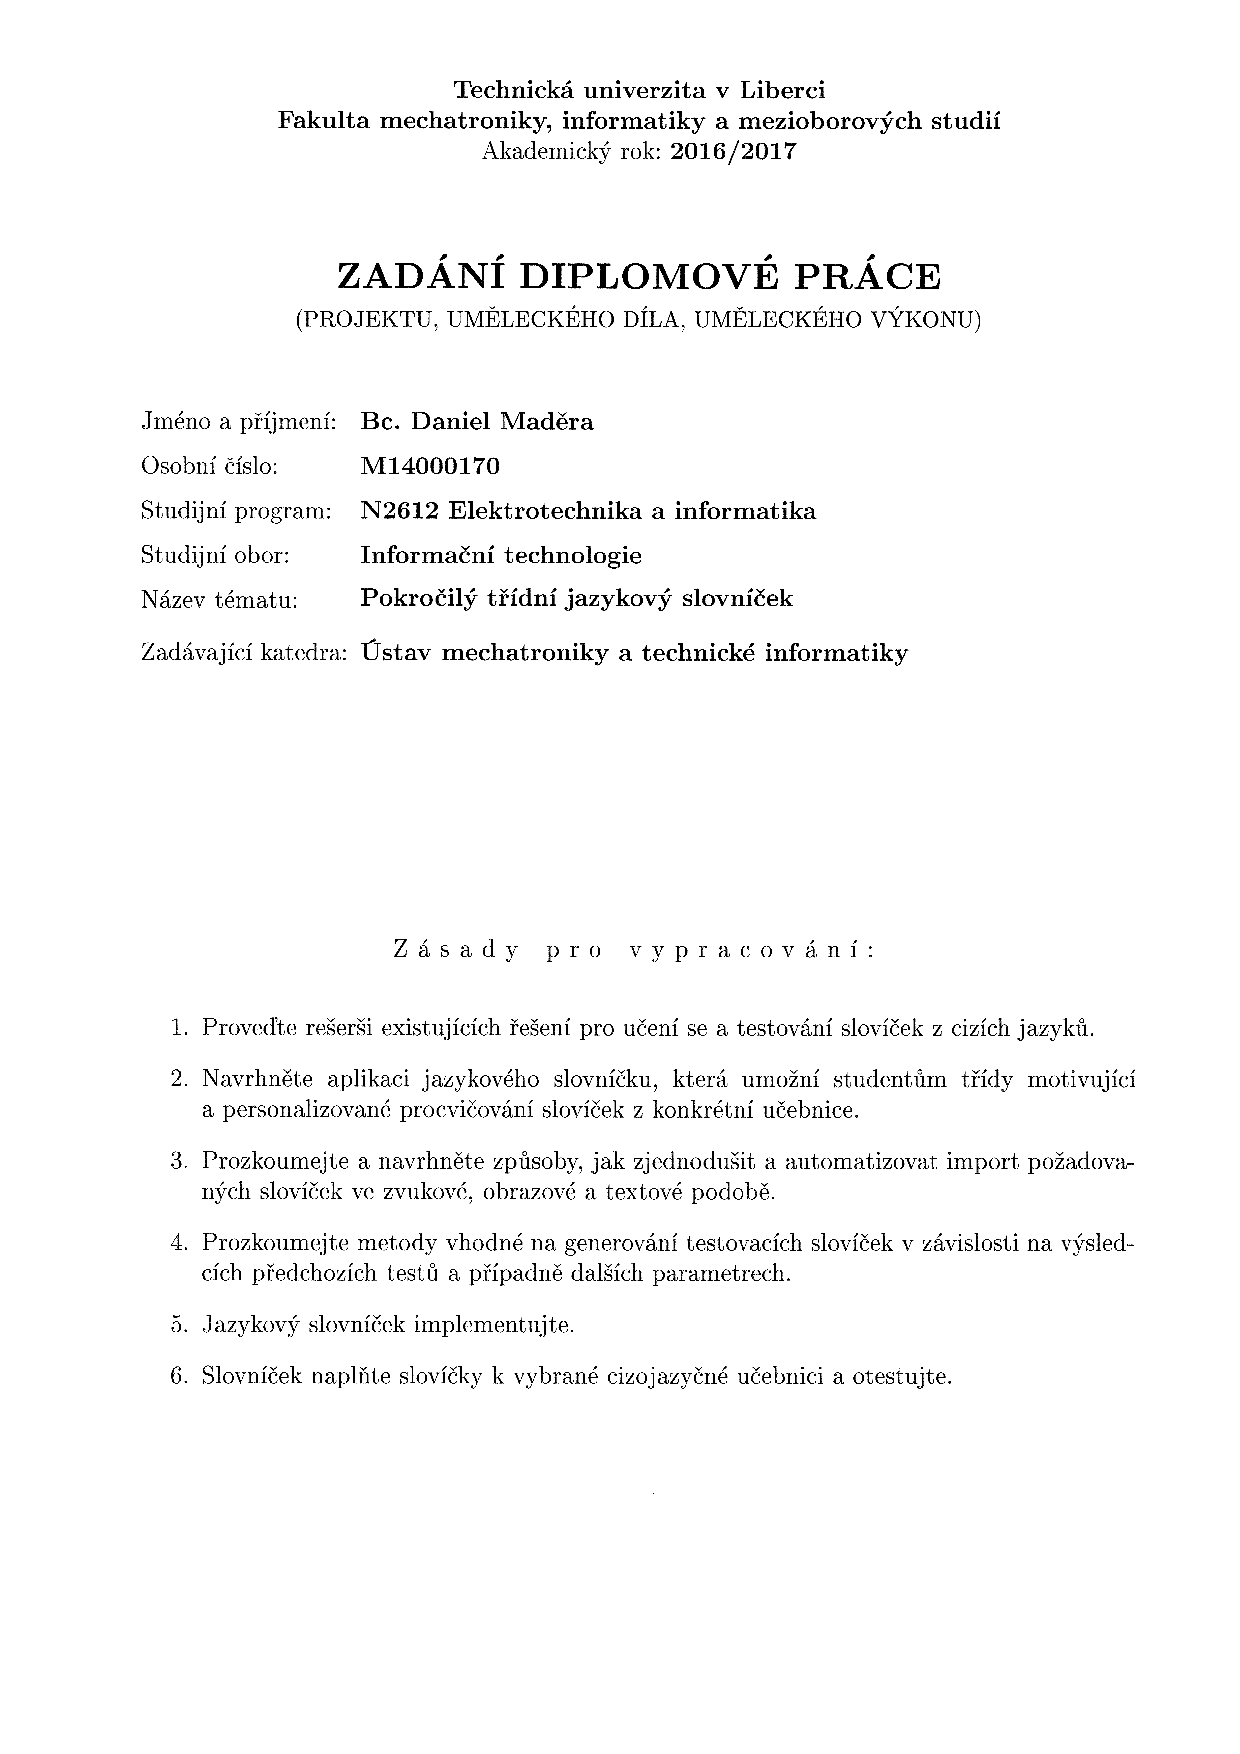
\includepdf[pages={1,2}]{zadani.pdf}

\includepdf{prohlaseni.pdf}
\setcounter{page}{3}

\newpage
\thispagestyle{plain}
\section*{Abstrakt}
% 250 až 500 slov

\section*{Klíčová slova}
% 5 klíčových slov

\thispagestyle{empty}
\newpage

\section*{Abstract}
% 250 až 500 slov

\section*{Keywords}
% 5 klíčových slov

\thispagestyle{empty}

\newpage
\thispagestyle{empty}
\setcounter{tocdepth}{2}
\tableofcontents


\newpage
\thispagestyle{empty}
\listoffigures
\listoftables
\renewcommand{\lstlistingname}{Ukázka kódu}
\renewcommand{\lstlistlistingname}{Seznam ukázek zdrojových kódů}
\lstlistoflistings

\newpage
\thispagestyle{empty}
\printglossary[title=Seznam zkratek]
\cleardoublepage

\section{Úvod}
    % proč se zaobývat tímto tématem
    % neopakovat abstrakt, lehce nastínit zadání, jaká je motivace
    % popsat, jak je práce strukturovaná - rozcestník


\newpage
\section{Analýza}
    Výuka cizích jazyků je pro aktuální společnost jedna z nejzásadnějších otázek, ať se jedná o pracovní příležitosti v zahraničí, tak sociální problematika světa. Žáci a studenti se často účastní různých kroužků nebo později studenti využívají Erasmus programů, kde vyhledávají právě zlepšení komunikace v cizím jazyce. 

    \subsection{Hlavní cíle}
        % jak si aplikaci představuji
        % zlepšení přípravy na hodiny cizího jazyka
        % shrnout v odstavci požadavky na aplikaci
        
        Hlavním cílem aplikace je připravit žáky na hodinu cizího jazyka a zároveň přirozeně rozvíjet slovní zásobu, tak aby studenti neztratili motivaci a chuť k poznávání nových výrazů. Dále také umožnit žákům se protestovat a ověřit, zda naučenou sadu slov ovládají. Aplikace by se měla adaptovat na zdatnost a úroveň každého ze žáků. Vyučujícím by aplikace měla usnadnit správu a import slovíček, které třída má umět v rámci dané učebnice a následně předkládat žákům vhodnou slovní zásobu například pro následující lekci.

        \subsubsection{Personalizace}
            % personalizace podle potřeby konkrétní třídy - konrétní učebnice
            % personalizace podle potřeby jednotlivých žáků - generování na základě předcházejících výsledků
            Důležitým cílem aplikace by měla být personalizace podle potřeby jednotlivých žáků a celých tříd. Personalizace na úrovni žáka znamená přistupovat individuálně na základě jeho úrovně znalostí a dovedností. V případě konkrétní třídy jde o individuální přístup a to zejména v sadě slov, které je třeba v přípravě procvičovat. 

        \subsubsection{Motivace}
            Důležitou součástí vzdělávání obecně je motivace. Tedy přimět žáky, aby z vlastní iniciativy chtěli rozvíjet své vědomosti. Problém ale je, že se děti přirozeně neučí z vlastní iniciativy, ale aby uspokojili okolí. Motivace se rozdělují do skupin - vnitřní a vnější nebo pozitivní a negativní \cite{bib:motivace}. V analýze bude zaměřeno pouze na motivační prostředky, které lze zařadit do aplikace pro procvičování slovíček.

            Motivace založená na základě vlastních úspěchů je důležitá pro utvrzení sebevědomí žáků. Ocenění v případě zvládnutí sady slov nebo gramatického bloku lze v případě aplikace implementovat například hláškami s projevem pochvaly nebo jiným upozorněním na dosažený výsledek. Zajímavým prvkem v aplikaci by mohlo být i herní prostředí. Žáci si rádi hrají a již J. A. Komenský poukázal na důležitost her ve vzdělávacím procesu.

            % motivace dětí k učení slov (vrámci třídy)
            % motivace - přispění k úspěchu třídy
            % motivace - vlastní úspěchy

            Jedním z dalších stěžejních faktorů motivace je kolektiv. Právě díky kolektivu, ve kterým funguje přirozená rivalita, jsou schopni žáci dosáhnout mnohem vyšších výsledků než kdyby se vzdělávali odděleně a samostatně. Rivalita a soutěživost může projevovat i velmi negativním způsobem. Místo kamarádských vztahů mezi dětmi mohou vznikat nepřátelské, kde může docházet i k posměchu těch, kteří nemusí mít pro výuku až takové nadání. Zajímavější motivací tedy pro kolektiv je například vidina společně dosažených výsledků. V případě učení slovíček by to byl počet slovíček naučených za rok jako celá třída. Dochází zde k utužování kolektivu a děti by mohlo těšit to, že nějakým způsobem přispívají k úspěchům celé třídy.

        \subsubsection{Využití IT pro výuku}
            Posledních několik let se společnost ubírá trendem informačních technologií. Každý ze žáků má už od útlého věku přístup k počítači nebo k chytrému telefonu. Orientace a schopnost tyto zařízení používat není pro ně žádný problém. Přirozeně se tedy tyto zařízení postupně stávají součástí každodenní přípravy žáka na následující školní den. V některých případech tyto zařízení plně nahrazují klasické učebnice a jsou přímo začleněny do výuky. Použití informačních technologií má za následek i zlepšení motivace při výuce. Obecně je známo, že žáci raději studují slovíčka interaktivní formou hádanek, křížovek nebo her, než nekonečných seznamů slov.

            Důležitost cizích jazyků se projevuje na míře používání například chytrých tabulí nebo tabletů při výuce. Tyto zařízení umožňují interaktivní výuku, kde lze využít nejen textových, ale také obrázkových a zvukových prostředků pro lepší zasazení nově nabytých vědomostí do kontextu. 

            % výuka cizích jazyků - smartboards            
            % vysoká motivace dětí pracovat s PC

    \subsection{Existující řešení}
        Na trhu lze nalézt nepřeberné množství aplikací pro výuku cizích jazyků. Řada z nich jsou téměř komplexní systémy, které provází studenta od základních frází a slovíček až po gramatické standardy cizího jazyka. Analýza existujících řešení byla zaměřena na aplikace, které se zabývají především testováním slovíček a frází.

        Do analýzy existujících řešení byly zahrnuty tři desktopové, jedna webová a jedna mobilní aplikace.

        \subsubsection{TS Angličtina}
            Z analyzovaných řešení se jevila desktopová aplikace TS Angličtina od firmy Terasoft ta nejlépe funkčně propracovaná. Tato firma se zabývám širokou škálou výukových nástrojů se zaměřením na základní školy. V případě cizích jazyků se zabývají výukou anglického a německého jazyka. Hlavní předností aplikace je podpora nejvíce používaných učebnic cizího jazyka. Aplikace umožňuje testování různými způsoby - psaný překlad slova, porozumění mluvenému slovu, vybírání správných významů nebo doplňování vynechaných slov \cite{bib:terasoft}. Analýza byla tvořena pouze z informací vydavatele. Bohužel firma Terasoft neposkytuje DEMO nebo TRIAL verzi aplikace, která by hlubší analýzu umožňovala.

        \subsubsection{Langsoft Teacher}
            Dalším analyzovaným řešením byla aplikace Langsoft Teacher, která je dostupná v podání desktopové aplikace, ale také i mobilní aplikace pro platformy iOS a Android. Aplikace je velmi komplexní, obsahuje různé moduly pro testování například v obrazové formě pro předškolní děti. Zajímavá vlastnost, kterou aplikace disponuje, je pamatování problematických slov a nabízení těchto slov častěji než těch bezproblémových. Dále program umožňuje automaticky rozšiřovat slovní zásobu, která je v testování zahrnuta \cite{bib:langsoft}.

        \subsubsection{Duolingo}
            Dalším v pořadí byla aplikace Duolingo. Jedná se o mobilní aplikaci pro Android. Zahrnuje učivo cizího jazyka od základních komunikačních frází až po tvorbu gramaticky složitějších vět. V aplikaci je připravena dlouhá řada cizích jazyků - němčina, angličtina, španělština (kastilština), italština a další. Chybí ale více referenčních jazyků. Aktuálně lze využít pouze angličtinu. Aplikace kromě standardních funkcí zahrnuje i rozpoznávání mluvených odpovědí. Zajímavým poznatkem byl systém motivace uživatelů, kde si každý mohl pozvat své přátele, mezi kterými docházelo k sdílení dosažených výsledků. Dalším motivačním základem bylo nutkání udržení plánu pravidelného testování, jelikož v opačném případě docházelo k automatickému zvyšování objemu testovacích dat. Nevýhodou aplikace byla nutnost připojení k internetu. V případě požití mobilních dat, docházelo ke zpoždění zejména při rozpoznání slov.

        \subsubsection{Vocabulary Trainer}
            Vocabulary Trainer je webová aplikace zdarma napsaná v jazyce PHP, která naučí 5000 nejvíce používaných slov daného jazyka. Aplikace umožňuje hodně možného nastavení. K dispozici je i řada jazyků včetně češtiny a to jako referenční i jako učený jazyk. Testování spočívá nejdříve ve čtení slov a následně uživatel vybírá možnosti odpovědi. Aktuálně překládané slovo si lze kdykoliv přehrát v různé rychlosti. Jako motivační základ aplikace využívá jednoduchý bodový systém. Součástí je i kalendář s email upomínkou k dalšímu testování. Program je propracovaný, ale poměrně pomalý a dlouho trvá zejména úvodní načítání dat. Její výrobce LanguageCourse S.L. poskytuje i mobilní aplikaci pro Android k učení anglických slov a frází.

        \subsubsection{Supermemo aplikace}
            \label{supermemo-app}
            Za zmínku ještě stojí aplikace Supermemo. Není to aplikace s připravenými daty k testování slov cizího jazyka, ale slouží čistě jako šablona pro testování jakéhokoliv druhu otázek. Aplikace implementuje algoritmus Supermemo, který je založen na metodě postupného zvyšování intervalu dotazování na dané otázky. Při každé odpovědi program spočítá, kdy by si uživatel měl danou otázku zopakovat tak, aby odpověď byla správná a zároveň se co nejvíce zvyšoval interval mezi aktuální a předchozí odpovědí. Aplikace se adaptuje na schopnosti uživatele, v přiměřeném měřítku buď zvyšuje nebo snižuje interval dalšího připomenutí.

        % možné ještě rozvést aplikaci EasyWords

        % žádná z aplikací neumožňuje personalizované učení 
        % ve škole (z učebnice) se učí jiná slovíčka než v aplikacích
        % po otestování slova nedochází k jeho znovu připomenutí

        Z výše uvedených aplikací až na Supermemo žádná neumožňuje personalizovaný výběr učiva. Tedy nelze vložit vlastní slovíčko nebo si určit sadu slov pro testování. Proto jsou tyto aplikace především cílené pro uživatele, kteří vnímají výuku jazyka jako samostatné vzdělávání sami sebe. Pro studenty, kteří absolvují lekce z cizího jazyka ve škole je tento typ vzdělávání nevyhovující, jelikož se musí učit dvě nezávislé skupiny slov. Sice dochází k rozvinutí slovní zásoby studenta i do jiných okruhů než je jeho učebnice a málokterý student má ještě energii, časovou dotaci a vlastní iniciativu na to, aby se připravoval na školní test ze slovíček a ještě rozvíjel samostatně svoji cizojazyčnou slovní zásobu.

    \subsection{Učení slovíček}
        % problematika malých dětí a učení slov
        % Biemiller and Boote (2006)
        % ročně se dá zvládnout maximálně 400 slov u studentů 2 - 5 třídy
        % docházelo k zvýšení učenlivosti, když studenti si mohli zapsat 
        % slovo vlastní definicí
        Standardní učení slovní zásoby cizího jazyka je založeno na častém opakování slov. Dle výzkumu Biemillera a Boote se lze ročně zvládnout až 400 slov u studentů 3.—6. tříd \cite{bib:beimiller}. Což v případě cizího jazyka poměrně velké číslo, ale problém je, do jaké míry je slovo správně ukotveno v dlouhodobé paměti. Porovnání, kolik je potřeba slov pro ovládnutí anglického jazyka, usnadní následující tabulka \ref{tab:english-vocab-usage}, která zahrnuje procentuální využití nejvíce používaných slov v každém z odvětví \cite{bib:learning-vocab}. 

        \begin{table}[ht!]
            \centering
            \begin{tabular}{|l|c|c|c|}
            \hline
            & \multicolumn{1}{l|}{Konverzace} & \multicolumn{1}{l|}{Noviny} & \multicolumn{1}{l|}{Akademický text} \\ \hline
            1. 1000 slov & 84,3\% & 75,6\% & 73,5\% \\ \hline
            2. 1000 slov & 6\% & 4,7\% & 4,6\% \\ \hline
            Akademické výrazy& 1,9\% & 3,9\% & 8,5\% \\ \hline
            Ostatní & 7,8\% & 15,7\% & 13,3\% \\ \hline
            \end{tabular}
            \caption{Používání slov v britském anglickém jazyce}
            \label{tab:english-vocab-usage}
        \end{table}

        \subsubsection{Zastaralý způsob učení}
            Dle vlastního průzkumu žáci základních škol nevyužívají k učení slovíček nikterak pokročilé technologie. Většinou si udržují vlastní slovníček, do kterého nově nabytá slova. Při učení zakrývají část s cizími slovy a na základě českého ekvivalentu se snaží vybavit překlad slova. Tato metoda neposkytuje prakticky žádnou zpětnou vazbu. Žáci většinou pouze do krátkodobé paměti uloží slova, později při testu rychle zodpoví a následně během pár hodin si na slovo už ani nevzpomenou. Nevýhod a námětů na zlepšení metody má tato metoda celou řadu, ale jedním z klíčových vad je, že žáci si nevytvoří dostatečně souvislostí, aby řádně ukotvilo slovo v paměti.

        \subsubsection{Zvuková interpretace}
            Zejména v učení cizího jazyka je zvuková podoba a interpretace slov velice důležitá. Jelikož každý jazyk může hlásky různě zvukově interpretovat a pro nováčka v cizím jazyku nemusí textová výslovnost plně vyhovovat. Žák dále díky znění slova získá podvědomí o dialektu daného jazyka a zároveň dochází k lepšímu zapamatování slova. Právě díky zvukům dochází k propojení při učení i pravé mozkové hemisféry. A napomáhá tedy k vytvoření pevnější ukotvení v paměti. Dle studie bulharského vědce George Lozanova, který se zabýval studiem mozku a učebních metod, byl zjištěn obrovský přínos zvukových vjemů \cite{bib:suggestology}.

        \subsubsection{Problematika obtížnosti}
            % každý z žáků má indiviální úroveň znalostí cizího jazyka
            % a každý z žádů se jiným tempem učí cizojazyčná slovíčka
            Velkým problémem v učení slov je přizpůsobit obtížnost každému ze žáků individuálně. Jelikož ne všichni mají stejnou úroveň znalostí cizího jazyka a každý potřebuje jiné tempo pro zapamatování sady slov. Jsou žáci s výbornou pamětí, kterým stačí si slova pouze jednou projít a dokáží je používat, ale jsou žáci, kde nestačí je pětkrát zopakovat. Dalším problémem obtížnosti je z pohledu jednotlivých slov. Každé slovo má odlišnou obtížnost, které lze soudit například podle míry používanosti v jazyce, délky slova, zdali obsahuje přehlasování, dvojitá písmena nebo podobnost s referenčním slovem.

        \subsubsection{Učení slov v kontextu}
            % jak je důlžité se slova učit v kontextu - použití ve větě z učebnice
            % drive/vocab-techniques.pdf
            Pro učení slov cizího jazyka je rovněž důležité správné zasazení významu slova do kontextu. Dle průzkumu Biemillera a Bootea z roku 2006 bylo zjištěno, že u žáků od 10—13 let docházelo k nárůstu zapamatovaných slov o 4\%, pokud byla slova předložena v kontextu vět. Důležitým poznatkem z toho průzkumu je, že žáci si nejen déle naučené slovo pamatovali, ale správně ho i interpretovali, když měli za úkol ho svými slovy vysvětlit \cite{bib:beimiller}. Ve stejném průzkumu rovněž docházelo ještě k vyššímu zlepšení v učení, kdy si žáci zapisovali vlastními slovy definici a použití slova. 
        
    \subsection{Testování slovíček}
        % drive/accesing-vocabulary-in-the-language-classroom.pdf
        % důležitost aktivní slovní zásoby pro výuku cizího jazyka

        \subsubsection{Aktivní a pasivní slovní zásoba}
            % co je aktivní a pasivní
            Slovní zásobu, kterou využíváme k tvorbě vět ať už v cizím nebo mateřském jazyce rozdělujeme na dvě skupiny - aktivní a pasivní. Pasivní zásoba je sada slov, která jsou pevně a spolehlivě uložena v naší paměti. Průměrný žák zná cca 50 000 výrazů. Její velikost je ovlivněna věkem, vzděláním a četbou. Slova ze této sady využíváme zejména při písemné formě, ať už se jedná o čtení nebo psaní. Aktivní zásoba je sada slov, ve které lze najít žádané slovo během desítek milisekund. U většiny lidí dosahuje velikosti 4 000 až 8 000 výrazů \cite{bib:lexikologie}. Slovo se díky používání dostává z pasivní do aktivní slovní zásoby. 

        \subsubsection{Metody testování}
            \label{test-methods}
            % pasivní vs aktivní
            % aktivní - vzpomenutí, rozpoznání

            Metod testování slovní zásoby je mnoho. Základním rozdělením je na pasivní a aktivní. V případě pasivního se jedná například o výběr z nabídnutých možností. Jde o případ, kdy student nemusí znát přesnou odpověď a dokáže otázku vyhodnotit správně vylučovací metodou. Při aktivním testování žáci musí odpověď znát, aby otázka byla vyhodnocena správně. Pasivní metoda má pozitivní vliv například na motivaci žáka, který u ní tolik netápe a za pomoci zdravého rozumu může test vyhodnotit správně. Problém ale vzniká při používání získaných a procvičených informací. V případě cizího jazyka lze pasivní slovní zásobu využít pro čtení a náslech, ale pro ovládnutí cizího jazyka je nedostatečná a tudíž nevhodná. 

            Dalším rozdělením pasivního a aktivního testování slovíček je rozpoznávání (\textit{recognition}) a vzpomenutí (\textit{recall}). Rozpoznávání spočívá v předložení cizího slova žákovi a pro správné zodpovězení musí najít český ekvivalent. Vzpomenutí je způsob testování opačným způsobem než rozpoznání. Tedy uživateli je předložen výraz v jeho mateřském jazyce a on musí nalézt správný výraz v cizím. Rozpoznání je z principu jednodušší pro uživatele než vzpomenutí. Lze ho tedy využít rovněž pro zvýšení motivace při procvičování slov. Ale pro ověření, zda je slovo ovládnuté či nikoliv je metoda rozpoznání také nedostatečná.

        \subsection{Typy testů}
            % multiplechoice, matching, completion, translation
            % vyžití her - problém je, že tento způsob většinou není ani efektivní, jelikož si procvičí například v případě doplňování písmen pouze pár slov za poměrně dlouhý čas

            V analýze existujících řešení bylo procvičování a testování slov interpretováno různými způsoby. Obecně by se typ testů dal rozdělit na tři kategorie - textové testy, multimediální a herní testy.

            \subsubsection{Textové testy}
                Textové testy se vyskytovaly například jako výběr z více možností nebo spojováním spolu souvisejících významů, jak už ale bylo uvedeno v kapitole \ref{test-methods}, jedná se o rozvíjení pasivní slovní zásoby. Zajímavějším typem testů je doplňování slov do vět a klasický překlad slova. Tyto typy rozvíjejí žádanou aktivní slovní zásobu. Standardně textové testy byly doplněny zvukovou interpretací cizího slova.

            \subsubsection{Multimediální a herní testy}
                Zajímavým využitím multimédií by mohlo být zahrnutí otestování výslovnosti. Tedy možnost nahrání odpovědi a následně by došlo k rozpoznání. Ale analýza a rozpoznání řeči není nikterak triviální záležitost. Dalším zajímavým řešením byly herní testy. Díky nimž docházelo k zvýšením motivace uživatelů. Problém je, že tento typ procvičování většinou není zas tolik efektivní, jelikož si uživatel procvičí například v případě doplňování písmen křížovky nebo známé hry \textit{Hangman} pouze pár slov za poměrně dlouhý čas.

        \subsection{Metoda rozloženého opakování}
            \label{spaced-repetition}
            % obecně o metodě 
            Až na výjmečné paměti je obecně známo, že pokud chceme informaci v paměti uchovat dlouhodobě, je nutné opakovaně připomínat. Pokud informace není vyžívána s největší pravděpodobností dojde ke ztráte této informace. V případě, že uživatel s touto informací pracuje častěji, výrazně navyšuje šance pro její zapamatování. Metoda rozloženého opakování (\textit{spaced repetition}) je učební technika založená na opakovaném připomínání informace s navyšujícím itervalem. Na začátku učebního procesu, jsou intervaly krátké například na hodinu, 4 hodiny nebo celý den. S postupem se tyto intervaly mohou zvyšují až na týdny a měsíce. Ideální systém rozploženého opakování nabídne zopakování informace před tím, než dojde k jejímu eventuálnímu nevzpomenutí.

        \subsubsection{Křivka zapomínání}
            Křivka zapomínání je graf exponenciálního charakteru, který znázorňuje za jak dlouho a s jakou pravděpodobností je možné si na nově nabytou informaci vzpomenout. První tuto křivku specifikoval už v roce 1885 Hermann Ebbinghaus. Na ose Y lze nalézt procentuální pravděpodobnost vzpomenutí na informaci, na ose X je čas. V čase 0 dojde k nabytí informace a spostupem času dochází k zapomínání. U průměrných pamětí dojde k potencionálnímu zapomenutí nové nesouvisející informace bez kontextu během pěti dní \cite{bib:ebbinghaus}.

            Následující obrázek \ref{fig:forgetting-curve} znázorňuje metodu rozloženého opakování na křivce zapomínání. V čase s 80\% pravděpodobností vzpomenutí na danout informaci dojde k znovu připomenutí informace. Křivka zapomínání se posune na ose Y a znovu dochází k postupnému zapomínání. Díky exponencionálnímu charakteru interval mezi jednotlivými opakováními narůstá také exponencionálně. V ideálním případě se posune exponenciála tak, že se bude limitně blížit 80\% hranici.

            \begin{figure}[ht!]
                \centering
                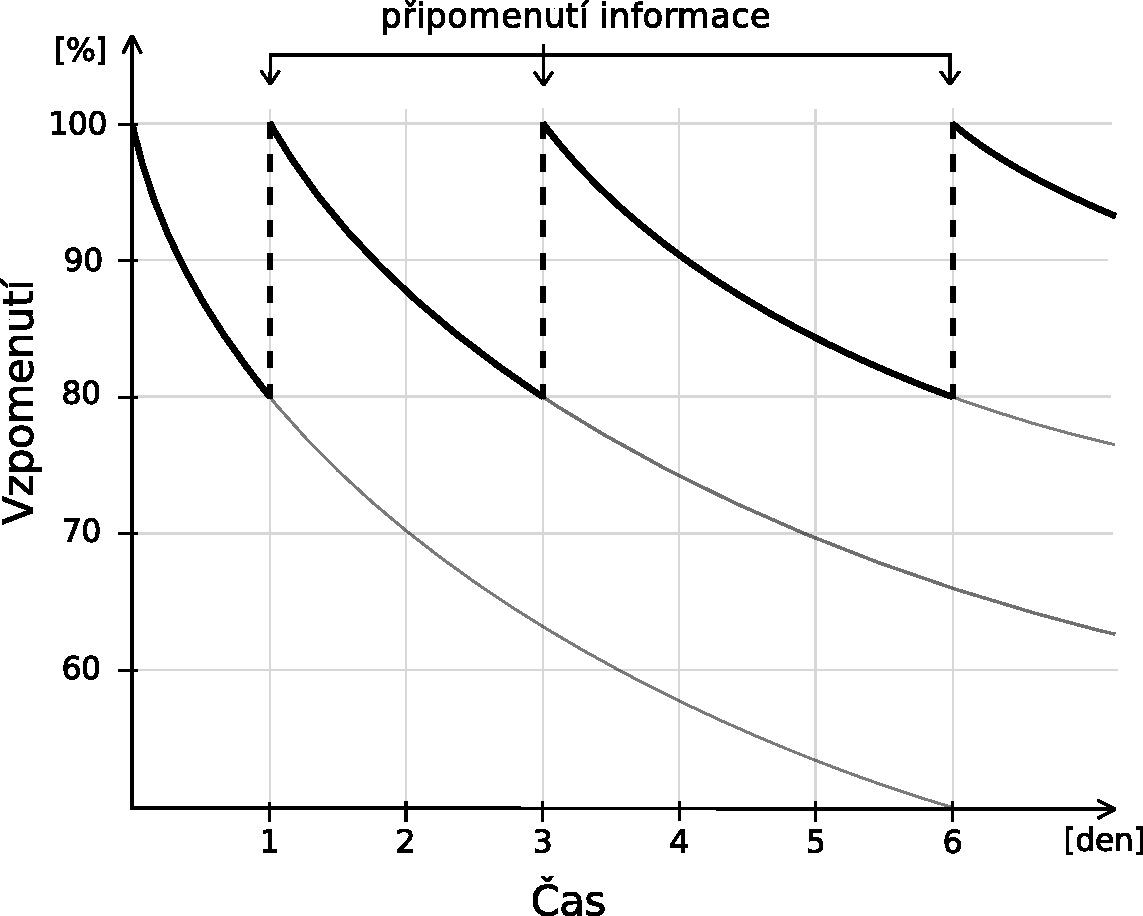
\includegraphics[scale=0.55]{../diagrams/forgetting-curve.pdf}
                \caption{Naznačení rozloženého opakování na základě křivky zapomínání}
                \label{fig:forgetting-curve}
            \end{figure}
         
        \subsubsection{Leitnerův algoritmus}
            % shrnout leitnerův algoritmus
            \label{leitner}
            Na Leitnerův algoritmus lze nahlížet jako na známý učební postup v podobě karet s otázkami na informace. Tyto karty jsou rozděleny do skupin, které jsou označeny například 1 až 3, kategorií ale obecně může být více. Nová karta je zařazena do první kategorie. Karty v první kategorii jsou opakovány častěji, v poslední kategorii jsou karty opakovány méně častěji. Karty jsou přemisťovány podle toho, jak uživatel zvládá odpovídat na jednotlivé otázky. V případě, že uživateli otázka na kartě nedělá problémy, přesune kartu do vyšší kategorie. V opačném případě, kdy uživatel nemůže opovědět správně na danou otázku, karta se přesune do prní kategorie a cyklus pro danou kartu začíná znovu.

    \subsection{Specifikace požadavků}
        % číselný seznam toho, co má aplikace dělat
        Na základě analýzy byla provedena specifikace požadavků, které budou implementovány v aplikaci pro testování slovíček z cizího jazyka.

        \begin{enumerate}
            \item správa učebnic
                \begin{itemize}
                    \item tvořit, editovat a mazat vlastní učebnice
                    \item umožnit publikovat učebnici pro veřejnost
                \end{itemize} 
            \item správa slovíček v učebnici
                \begin{itemize}
                    \item tvořit, editovat a mazat slovíčka
                    \item hromadně slovíčka do učebnice importovat
                    \item částečně automatizovat zvukovou a obrazovou interpretaci slovíčka
                \end{itemize} 
            \item správa modulů a tématických okruhů v učebnici
                \begin{itemize}
                    \item tvořit, editovat a mazat moduly a tématické okruhy učebnice
                    \item přiřazovat slovíčka do daných modulů a okruhů
                \end{itemize}
            \item správa uživatelských skupin (tříd)
                \begin{itemize}
                    \item tvořit, editovat a mazat uživatelské skupiny
                    \item umožnit uživatelům se přihlásit do skupiny
                \end{itemize}
            \item správa testovacích sad
                \begin{itemize}
                    \item tvořit, editovat a mazat testovací sady
                    \item umožnit vybírat slova pro testovací sadu z vlastních i veřejných učebnic
                    \item přiřazovat testovací sady ke skupinám uživatelů
                \end{itemize}
            \item procvičování slovíček
                \begin{itemize}
                    \item vybrat testovací sadu slovíček
                    \item generovat slova na základě úrovně uživatele
                    \item zahrnout obrazovou a zvukovou interpretaci do procvičování
                    \item možnost uložit stav testování a umožnit pozdější navázání
                \end{itemize}
            \item připomínat a procvičovat ovládnutou slovní zásobu 
            \item motivace
                \begin{itemize}
                    \item motivovat v rámci uživatelské skupiny
                    \item motivovat vlastní iniciativu k procvičování
                \end{itemize}
        \end{enumerate}


\newpage
\section{Návrh aplikace}
    % usecase diagram
    % jednotlivé use-case by měly být názvy jednotlivých podkapitol v návrhu aplikace
    Na základě specifikace požadavků byl vytvořen USE-CASE diagram aplikace. Diagram na obrázku \ref{fig:use-case} znázorňuje pouze obecné bloky funkčnosti aplikace. V následujících kapitolách bude každý z jednotlivých USE-CASE bloků popsán detailněji.

        \begin{figure}[ht!]
            \centering
            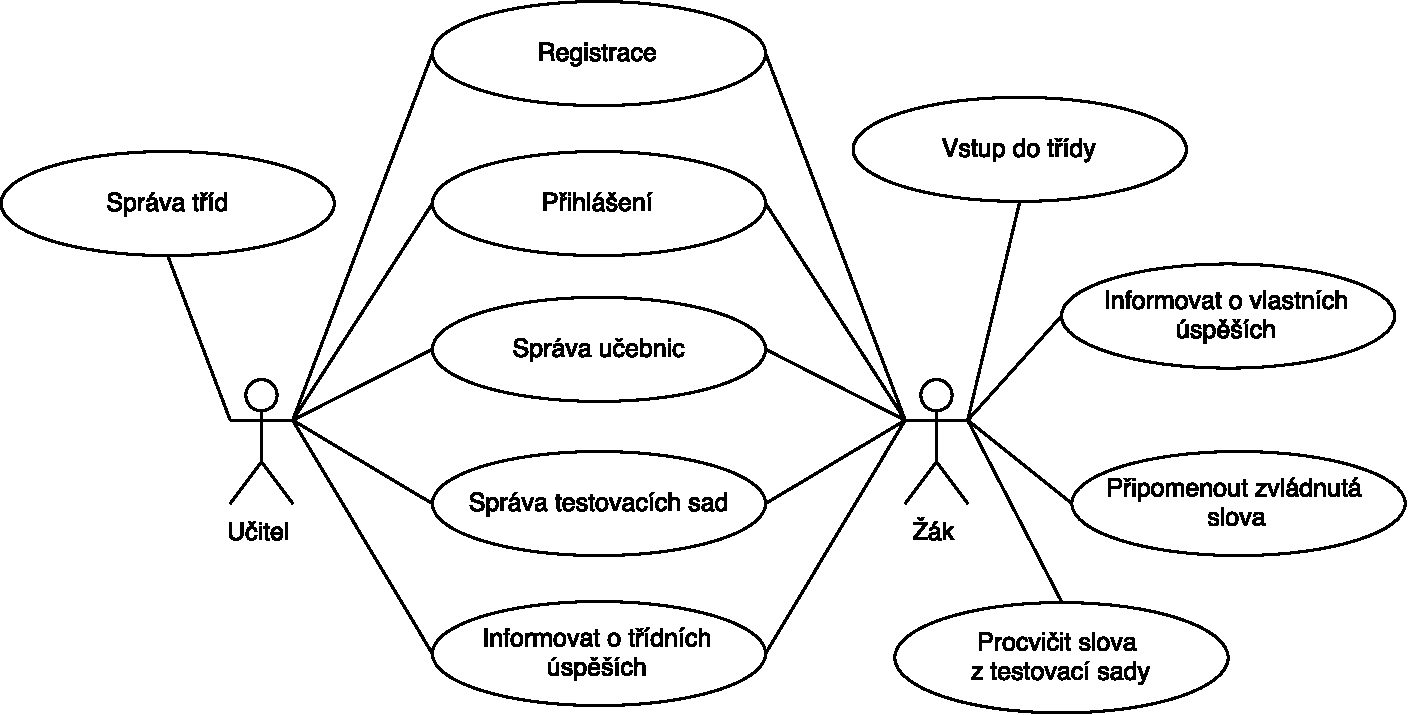
\includegraphics[scale=0.63]{../diagrams/use-case.pdf}
            \caption{USE-CASE diagram aplikace}
            \label{fig:use-case}
        \end{figure}

    \subsection{Uživatelské role}
        % rozvést rozdíl mezi žákem a učitelem - rovnocenné partnerství, každý může být učitel a student
        Do aplikace by měly vstupovat dva typy uživatelů - učitel a žák. Učitel z principu má za úkol spravovat testovací sady, učebnice a třídy. Žáci oproti nim mají za úkol vstupovat do svých tříd, procvičovat slova z testovacích dat, které jsou připravené od učitele a připomínat si zvládnutá slova. 

        Po konzultacích s vedoucím práce a vyučujícím cizího jazyka na základní škole došlo k několika změnám v návrhu právě v oblasti uživatelských rolí a i v principu aplikace. Vznikl požadavek, že aplikace by mohla fungovat spíše jako portál pro vzdělávání a ne jako výukový nástroj pro učitele. V návrhu tudíž vzniklo rovnocenné partnerství mezi učitelem a žákem.

        \subsubsection{Sjednocení uživatelským skupin}
            Podnětem pro sjednocení uživatelských skupin vedlo umožnění žákům procvičovat si slova i v případě, že nejsou součástí žádné třídy. Tak aby mohl kdokoliv se do aplikace přihlásit, vybrat si testovací sadu a vyzkoušet svoje znalosti slovíček. Tato funkce umožňuje žákům volnější přístup k výuce. Nebylo totiž v požadavcích to, aby učitel měl přehled o znalostech žáka - právě naopak. Účelem aplikace je poskytnout žákům možnost se samostatně vzdělávat a procvičovat slovní zásobu a ne vyučujícím poskytnout nástroj pro otestování, zda žák disponuje požadovanými znalostmi. 

    \subsection{Správa učebnic}
        % sdílení učebnic (otevřený systém)
        % přijít do aplikace a jen tak si protestovat slova z učebnice
        % nemusí být člověk součástí žádné skupiny
        Z důvodu personalizace slovíček bylo nutné v návrhu aplikace zařadit učebnice, díky nimž si žáci budou procvičovat pouze slovíčka, která jsou pro ně aktuální ve výuce cizího jazyka. Učebnice obsahují moduly a v modulech se nacházejí jednotlivá slova. Při tvorbě učebnice bude zvolen cizí jazyk, pro který je učebnice připravená. V rámci jedné učebnice jsou slova unikátní. Tzn. do konkrétní učebnice nemohou patřit dvě stejná slova. Majitel učebnice je může editovat, vytvářet, skrýt pro veřejnost a mazat i v případě, že je využívána některým z ostatních uživatelů. 

        V aplikace se může vyskytovat i více stejných učebnic. Například dva různí vyučující vedou své hodiny cizího jazyka dle stejné učebnice, ale každý si chce přizpůsobit sadu slov po svém. Proto se v aplikaci musí učebnice identifikovat majitelem a názvem učebnice.

        \subsubsection{Sdílení učebnic}
            Jelikož aplikace slouží jako portál pro vzdělávání, ve výchozím stavu jsou učebnice a slovíčka v nich veřejně přístupné jakémukoliv uživateli. Příchozí uživatel si tedy bude moci buď vytvořit vlastní učebnici se svými slovy, které si chce procvičit nebo může vyhledat už z vytvořených učebnic. Díky sdílení nový uživatel může prakticky okamžitě po přihlášení začít procvičovat slova a nemusí složitě žádná slova importovat. Tento přístup je cílený právě především pro žáky, kteří si chtějí samostatně procvičovat slova a nepatřit do žádné konkrétní třídy.


    \subsection{Správa slovíček}
        % výhody více forem - lepší zapamatovatelnost
        % vytvoření hlubších asociací

        Jednotlivá slovíčka se budou ukládat do daným modulů učebnice. Slovíčko se bude charakterizovat - překladem v cizím jazyce, významem v mateřském jazyce, definice slova v cizím i mateřském jazyce a použití ve větách z učebnice. Dalšími atributy, kterými slovíčko bude disponovat, jsou obtížnost a slovní druh. Slovíčko bude možné doplnit o multimediální interpretaci a to v podobě zvuku a obrázku.

        %% Možné rozšíření - přidat možnost více významů slova
        \subsubsection{Textová forma}
            % importováním sady slov (bez automatizace překladů)
            % editace definic a použití ve větách
            Textová forma slovíčka spočívá v překladu slova a jeho významu v mateřském jazyce. Pro zjištění významu slova se může využít již hotové aplikace. Například Google Translate poskytuje aplikační rozhraní pro překlady slov i celých vět. Výhodou by bylo usnadnění zadávání a import slovíček do aplikace. Jelikož se aplikace bude zabývat aktivním rozpoznání a vzpomínání, je vhodné neautomatizovat významy slov. Učebnice nebo učitelé se mohou s Google Translate lišit v definování významů slov. Dalším problémem je cena využívání překladů z Google Translete, která je účtovaná měsíčně a to \$20 za 1 milion znaků \cite{bib:google-api}.

        \subsubsection{Zvuková forma}
            % z Google API importovat zvukové nahrávky
            % shrnout omezení, problematiku
            % 60 minut měsíčně je zdarma
            Do aplikace by měla být implementována i zvuková interpretace slovíčka v cizím jazyce. Zvukové nahrávky mohou být zařazeny do aplikace dvěma způsoby - manuálně vlastními nahrávkami nebo využít Google Text to Speech API, které poskytuje zdarma, pokus se měsíční využití zvukových nahrávek obsáhne do 60 minut\cite{bib:google-api}. V případě jedno nebo dvouslovných spojení, které zaberou přibližně 4—8 vteřin, je dostačující pro cca 600 slovíček za měsíc. Aplikace bude záznam lokálně ukládat, aby bylo se co nejvíce omezilo využívání API. Zvuková nahrávka bude získána při importu slovíček do učebnice. Zadávající uživatel si bude moci zvolit, k jakému slovu chce zvukovou interpretaci.

        \subsubsection{Obrazová forma}
            % vyhledání z Google Images API na základě cizojazyčného slova
            % autor učebnice vybírá dané slovo z importovaných
            % omezení dotazů - neprovádí se plně automatiky
            Obrazová interpretace slovíčka bude rovněž získaná z Google Custom Search API. Toto aplikační rozhraní není omezené a lze v parametrech omezit vyhledávání pouze na obrázky. Při importu si uživatel zvolí pro jaká slovíčka chce obrazovou formu. Automatizace v tomto případě není vhodná, jelikož ne všechny slovíčka lze interpretovat jako obrázek. Uživatel si také bude moci zvolit obrázek z několika možností. Po vybrání obrázku bude vytvořena komprimovaná kopie souboru a uloží se rovněž zdroj, odkud je obrázek získán. Tato forma bude v aplikaci sloužit pouze jako nápověda pro žáky, díky níž si mohou ke slovíčku vytvořit hlubší asociaci. 

            % využití možnost hledání dle "Lze volně užívat nebo sdílet". Vytvoření kopie, 
            Díky Google Custom Search API lze vyhledávání parametrizovat. Výrazem pro vyhledávání bude referenční slovo v cizím jazyce, jelikož cílový jazyk bude nejspíš anglický, německý nebo španělský a všechny tyto jazyky jsou více rozšířené než ten český. Dalším parametrem vyhledávání je omezení pouze na obrázky s licencí a \uv{Volně užívat nebo sdílet}, která umožňuje obrázek zkopírovat a nekomerčně publikovat s uvedením zdroje. Bohužel společnost Google Inc. nezaručuje pod jakou licencí obrázek aktuálně se na stránkách prezentuje. Proto bude uživatel při výběru obrázku vyzván, aby zkontroloval licenci použití.

    \subsection{Obtížnost slovíček}
        % vygenerovaná obtížnost na základě délky slova, podobnosti s českým jazykem, přizpůsobena vyučujícím
        Při zadávání slova do učebnice bude automaticky vyhodnocena jeho obtížnost, která je rozdělena do čtyř kategorií - snadné, střední, těžké a nemožné. Vyhodnocení obtížnosti je založeno na kombinaci několika parametrů slova - jeho délky, podobnosti s českým ekvivalentem a další atributy jako počet přehlasovaných písmen nebo počet výskytů dvojitých písem. V případě nevhodně vygenerované obtížnosti slova, uživatel ji bude moci opravit dle vlastního uvážení. Délka slova je prahově rozdělena do kategorií obtížnosti, následně bude vyhodnocena podobnost s významem pomocí Levensteinovy vzdálenosti popsané v podkapitole \ref{levenstein}. Poté následuje vyhodnocení přehlasování a dvojitých hlásek, které ale ovlivňují obtížnost už minimálně.

        \subsubsection{Výběr algoritmu}       
            Levenshteinova vzdálenost je velmi podobná známe Hammingově vzdálenosti s tím rozdílem, že Hammingova vzdálenost uvádí počet pozic se stejným symbolem v obou řetězcích. Kdežto Levenshteinova uvádí počet jednoznakových editací. Pro určení míry podobnosti mezi slovem v cizím jazyce a jeho překladem je vhodnější Levenshteinova vzdálenost, jelikož akceptuje řetězce s různou délkou a v případě, že písmeno chybí, je to vyhodnoceno pouze jako odstraněné písmeno a algoritmus pokračuje dál. V případě Hammingovy vzdálenosti, vynechané písmeno naruší porovnávání zbytku řetězce.

        \subsubsection{Levenshteinova vzdálenost}
            \label{levenstein}
            Levenshteinova vzdálenost v informatice je míra rozdílu mezi dvěma řetězci. Pro výpočet vzdálenosti se využívá matice s rozměry velikostí délek řetězců. V podstatě vzdálenost je minimální počet jednoznakových úprav ve slově, aby vzniklo slovo referenční. Za jednoznakovou úpravu se považuje smazání, záměna nebo vložení písmene na dané místo.

            Vzorec \ref{levenshtein} je matematický zápis Levenshteinovy vzdálenosti, kde $a$ a $b$ jsou řetězce $a(i)$ a $b(j)$ jsou indexované znaky v řetězcích. Výsledná vzdálenost je rovna hodnotě v matici $dist_{a,b}$ na pozici $dist_{a,b}(|a|,|b|)$, kde $|a|$ a $|b|$ jsou délky řetězců \cite{bib:levenshtein}.

            \begin{ceqn}
            \begin{align}
                \label{levenshtein}
                dist_{a,b}(i,j) = 
                \begin{cases} 
                    max(i,j) & min(i,j) = 0\\min
                        \begin{cases}
                            dist_{a,b}(i-1,j)+1\\dist_{a,b}(i,j-1)+1\\dist_{a,b}(i-1,j-1)+
                            \begin{cases}
                                0 & a(i) = b(j)\\1 & a(i) \neq b(j)
                            \end{cases} 
                        \end{cases} & min(i,j) \neq 0 
                \end{cases}
            \end{align}
            \end{ceqn}

            V případě, že se pohybujeme v matici v prvním sloupci a prvním řádku přiřazujeme hodnoty 1 až délka řetězce $a$ do sloupce a 1 až délka řetězce $b$ do řádku. Tedy první sloupec a první řádek v matici slouží jako referenční inicializace. V generování matice se následně pokračuje a porovnávají se jednotlivé znaky. První položka v minimu je případ, kdy písmeno bylo odstraněno z $a$. Druhá položka je případ, kdy došlo k vložení znaku do a na základě znaku v $b$ řetězci. A poslední položka je případ porovnání znaků. V okamžiku, kdy znaky se rovnají, hodnota vzdálenosti na diagonále zůstává, v opačném případě se přičítá jednička.

            Výpočet Levenshteinovy vzdálenosti dvou slov znázorňuje matice \ref{leven-matice}, kde dochází k porovnání českého slova \textit{cyklus} a anglického výrazu \textit{cycle}. Tučně je znázorněna cesta výpočtu. Prováděné jednoznakové operace jsou žádná, žádná, žádná, záměna, záměna a vložení.

            \begin{ceqn}
            \begin{align}
                \label{leven-matice}
                \begin{matrix}
                    &  & c & y & c & l & e \\
                    & \textbf{0} & 1 & 2  & 3 & 4  & 5 \\
                    c & 1 & \textbf{0} & 1 & 2 & 3 & 4 \\
                    y & 2 & 1 & \textbf{0} & 1 & 2 & 3 \\
                    k & 3 & 2 & 1 & \textbf{1} & 2 & 3 \\
                    l & 4 & 3 & 2 & 2 & \textbf{1} & 2 \\
                    u & 5 & 4 & 3 & 3 & 2 & \textbf{2} \\
                    s & 2 & 5 & 4 & 4 & 3 & \textbf{3} \\ 
                \end{matrix}
            \end{align}
            \end{ceqn}

        \subsubsection{Určení globální obtížnosti}
            % shrnutí o váženém průměru obtížnosti, jaké a v jaké váze faktory jako Levenshtein, přehlasování a dvojitá písmena tvoří určení obtížnosti slova
            Základním parametrem globální obtížnosti slova je jeho délka, která má váhu 4 v celkovém průměru jednotlivých hodnot obtížnosti. Na základě prahových hodnot je délka rozdělena do čtyř kategorií - $\langle1,6)$ je snadné, $\langle6,11)$ je střední a $\langle11,\infty)$ je slovo těžké. Dalším parametrem k určení obtížnosti je Levenshteinova vzdálenost mezi referenčním slovem a jeho překladem, jejíž váha je 2. Znovu zde figurují nastavitelné prahové hodnoty - v případě, že se procentuální podobnost (tj. $pp = (1-a/l)*100$; kde $l$ je délka slova a $a$ je počet jednoznakových editací) nachází v intervalu $\langle70,100\rangle$, je obtížnost nejlehčí; v intervalu $\langle30,70)$ je střední a v intervalu $\langle0,30)$ je slovo těžké. Přehlasování znaku a dvojitý výskyt stejného znaku mají oba stejnou váhu 1. Bez výskytu přehlasování a dvojitého znaku je obtížnost kvalifikována jako snadná, jeden výskyt je střední obtížnost a více výskytů je obtížnost vyhodnocena jako těžká.

    \subsection{Generování slov pro procvičování}
        % generování slov na základě motivace, obtížnosti 
        % základem je slova, která jsou problematická pro žáka generovat častěji než slova, 
        % která zvládá s přehledem
        % účel generování slov má procvičit slova tak, aby byly správně ukotveny v dlouhodobé paměti a ne pouze v té krátkodobé
        Způsob generování slov je důležité pro správné ukotvení slova v dlouhodobé a ne krátkodobé paměti. Při testování bude docházet i k několika násobnému opakování slova. Základem generování je častěji a vícekrát předkládat slova, která jsou pro žáka problematická a slova, která jsou zvládnuta žákem s přehledem, jsou méně častěji testována. Pro generování byla zvolena metoda rozloženého opakování v podobě přizpůsobeného Leitnerova algoritmu, který je popsán v kapitole \ref{leitner}.
        
        Algoritmus pro procvičování slov se dělí na dvě části. V první části se zjišťuje, jaká slova jsou pro zkoušeného uživatele jednoduchá a naopak s jakými slovy má problém - tato fáze se bude dále nazývat inicializační. Po této fázi následuje fáze s použitím Leitnerova algoritmu - tato fáze bude nazývána testovací.

        \subsubsection{Inicializační fáze}
            \label{init-faze}
            % setřídění slov nejlehčí, nejtěžší atd.
            % na základě odpovědi určení počet nutných správných opakování
            Na začátku testování jsou k dispozici slova s přiřazenou obtížností. Tato obtížnost je buď globální v případě, že se uživatel nesetkal ještě s daným slovem v aplikaci nebo uživatelská v případě, že uživatel dané slovo již procvičoval. Dle této obtížnosti se slovíčka seřadí tak, aby se střídala nejnižší a nejvyšší obtížnost. Na prvním místě tedy je slovo s nejnižší obtížností, následuje slovo s nejvyšší, dále slovo s druhou nejnižší atd. Důvodem tohoto seřazení je zvýšení motivace dětí. V případě, že by žák dostal na začátku nejtěžší slova, mohlo by si vytvořit odpor k procvičování v domnění, že slova jsou příliš složitá pro něj. 

            Uživatel tedy postupně odpovídá na slovíčka. Jeho odpověď je vyhodnocena buď správně, špatně nebo neúplně. Na základě vyhodnocené odpovědi a globální nebo uživatelské obtížnosti je ke slovu přiřazen počet správných opakování pro dokončení slova.

        \subsubsection{Testovací fáze}
            % výběr slov na základě Leitnerova algoritmu
            Po inicializační fázi následuje fáze testovací. V této fázi již je známo, jaká slova dělají uživateli problém. Oproti standardnímu Leitnerovu systému popsaném v kapitole \ref{leitner}, kde na začátku jsou všechny otázky zařazeny do první kategorie, zde se otázky rozdělují do třech kategorií na základě inicializační fáze. Následuje první fáze, kde dochází postupnému procházení otázek v první Leitnerově kategorii od nejtěžší pro uživatele po nejlehčí. V případě správně nebo neúplně zodpovězené otázky, slovo je přesunuto do vyšší kategorie. Následuje druhá fáze, kde se prochází otázky z první a druhé Leitnerovy kategorie. I zde platí, na základě odpovědi dochází k přesouvání otázek mezi kategoriemi, jak už tomu je ve standardním provedení Leitnerova systému. Ve třetí fázi jsou nabízeny otázky z první, druhé a třetí Leitnerovy kategorie. Po průchodu třetí fáze následuje znovu fáze první. Takto algoritmus cykluje do doby, dokud uživatel nepřeruší test nebo nezůstanou žádná slova, které by uživatel nedokončil. 

            Za dokončené slovo se považuje takové, kde uživatel odpověděl správně nebo neúplně tolikrát, kolik má slovo přiřazených nutných správných opakovaní, a zároveň poslední odpověď nesmí být neúplná, ale pouze správná. Je to z důvodu, aby bylo ověřeno, že uživatel má správně zapamatovanou informaci.

            % možná nějaký obrázek 

        \subsubsection{Adaptivní a globální obtížnost}      
            % ukládání Leitnerovy kategorie jako adaptivní obtížnost
            V případě přerušení testu dochází k ukládání aktuální Leitnerovy kategorie k danému uživateli. Díky tomu lze znovu navázat v případě, že uživatel se bude chtít k testování dané skupiny slov vrátit. Leitnerova kategorie vypovídá, jak problematické je slovo pro uživatele. V případě, že se slovo nachází v první kategorii je problematické a v případě, že se nachází ve třetí, uživatel ho zvládá bez obtíží. Díky této informaci dochází k adaptivnímu generování obtížnosti. V případě, že není u daného slova a uživatele uložená Leitnerova kategorie, je v inicializační části brána globální obtížnost.

            Například se může stát, že globální obtížnost slova je v kategorii těžkých, ale uživatel se s tímto slovem už několikrát setkal a dobře se mu pamatuje. Je proto zbytečné slovo mu opakovat vícekrát, jelikož na základě obtížnosti a správnosti odpovědi se generuje počet opakování. 

    \subsection{Procvičování slovíček}
        % učitel nevidí statistiky dětí, pouze celé třídy
        % aplikace nemá sloužit na zkoušení dětí učitelem
        % testing to learn, not testing to assess 
        Základní myšlenkou procvičování a testování slovíček je pomoci se žákům efektivně naučit slovíčka, nikoliv poskytnou vyučujícím možnost posuzovat, jak na tom žáci jsou. Následující podkapitoly popisují, jakým způsobem probíhá testování, napovídání, vyhodnocování odpovědí a kontrola podvádění.

        \subsubsection{Metody testování}
            % aktivní rozpoznání a aktivní vzpomenutí
            % algoritmus na záměnu vzpomenutí a rozpoznání (možná obrázek)
            Pro procvičování slovíček je zvolen pouze aktivní přístup a to v metodách aktivního rozpoznání a aktivního vzpomenutí. Tyto metody se automaticky střídají v závislosti na odpovídání uživatele. V případě inicializační fáze procvičování, popsané v kapitole \ref{init-faze}, se metoda testování nemění, aby uživatel měl stejné podmínky pro vyhodnocení úvodní obtížnosti slova. V následující fázi, kde probíhá samotné procvičování se metody střídají. Když uživatel odpoví špatně na vzpomenutí a u slova má více než jednu nutnou správnou odpověď pro dokončení slova, následující procvičení stejného slova je metodou rozpoznání. Je to z důvodu zvýšení motivace, aby procvičování uživatele neodradilo, když si nevzpomene na cizojazyčný výraz. 

            Jelikož vzpomenutí je paměťově náročnější úkol pro uživatele, je nutné, aby metoda potencionálně poslední odpovědi byla vzpomenutí. Jinak není možné ověřit, zda uživatel opravdu se slovo naučil i v cizojazyčném výraze. Tzn. V případě, že počet nutných správných odpovědí byl vyhodnocen na číslo 2, první metoda testování bude rozpoznání - uživatel napíše význam slova v mateřském jazyce. Pokud odpoví správně následuje metoda vzpomenutí. Pokud ale odpoví špatně, následuje znovu metoda rozpoznání.
    
        \subsubsection{Nápovědy}
            % definice se zobrazuje ihned, kontext slova ve větě z učebnice, první písmeno
            % možnost vyplnění definice slova - (automaticky předvyplnit - volně dostupné definice)
            V procvičování slovíček uživatel má k dispozici i nápovědy, v případě, že vlastník učebnice vyplní ke slovům i doplňující informace jako definici a použití ve větě z fyzické učebnice. Tyto nápovědy jsou použity pouze v případě, že se testuje metodou vzpomenutí. Další nápovědou je zobrazení prvního písmene odpovědi. Definice je nápověda, kterou uživatelé vidí jako doplňující atribut otázky. V případě, že uživatel klikne na tlačítko "Použít nápovědu", zobrazí se mu první písmeno odpovědi. Pokud klikne na tlačítko znovu, zobrazí se mu použití slova ve větě.

        \subsubsection{Vyhodnocování odpovědí}
            % určení vzdálenosti slov - více úrovní odpovědí
            % využívá se Levenshteina
            K vyhodnocování odpovědi se využívá znovu Levenshteinovy vzdálenosti popsané v kapitole \ref{levenshtein}. Odpověď je vyhodnocena do tří kategorií - správně, špatně a neúplně. Před porovnáváním slova, je z odpovědi odstraněné mezery, tabulátory a další speciální znaky. Správně je vyhodnocena pouze odpověď, která se plně shoduje s referenčním slovem. Jako neúplná je vyhodnocena v případě, že na 5 písmen je pouze jedna jednoznaková editace - tedy chybovost 20\%. V ostatních případech je odpověď vyhodnocená jako špatná. Pokud uživatel využije alespoň jednu z nápověd, automaticky se vyhodnocuje odpověď jako neúplná i v případě zcela správné odpovědi. 

        \subsubsection{Kontrola podvádění}
            % problém, není možné kontrolovat, zda si uživatelé nevyhledávají
            % slova ve slovnících a potom nedoplňují do aplikace
            % měření času odpovědi - v závisloti na délce odpověd 
            Aplikace nemá za úkol testovat žáky, zda zodpovědně a bez pomoci procvičují slova. Filozofie aplikace má být motivovat žáky a poskytnout jim příjemný nástroj na efektivnější učení slovíček z cizího jazyka. Proto v aplikace nejsou zakomponovány žádné mechanismy, které mají za úkol kontrolovat uživatele, zda si například nevyhledávají slovíčka ve slovníku nebo nepracují na procvičení společně s další osobou. 

            Jsou způsoby, jak by se ale tato funkčnost dala do aplikace implementovat a to například v podobě měření času odpovědi. Vyhodnocení by bylo na základě délky odpovědi a časem odpovědi. Další, více striktnější, omezení podvádění by mohla být kontrola, zda uživatel opustil aktuální okno aplikace.

    \subsection{Připomínání slov}
        % shrnout supermemo aplogritmus
        Připomínání slov je důležitou součástí aplikace. Funkce slouží k tomu, aby studenti nezapomněli na již naučená a zvládnutá slova z procvičování. Jelikož se jedná o webovou aplikaci, není úplně možné připomínat slova v přesných intervalech přímo v aplikaci. Způsob implementace připomínání slov je závislý na tom, aby se uživatel sám přihlásil a spustil funkci připomínání slov. Je možné na základě softwarového démonu Cron v určitých intervalech ze serveru odesílat emailová upozornění se slovy, které by si měl uživatel připomenout.

        \subsubsection{Supermemo algoritmus}
            Supermemo algoritmus je rovněž další implementace metody rozloženého opakování popsané v kapitole \ref{spaced-repetition}. První implementace Supermemo algoritmu v papírové podobě byla vytvořena již v roce 1985. V aplikaci je využívání aktuální verze 11, poprvé implementována v roce 2005. 

            Algoritmus má dvě možnosti implementace - optimální interval a pokročilé opakování \cite{bib:supermemo}. Verze s optimálním interval je pro účely aplikace dostačující, jelikož pro implementaci s pokročilým opakováním by bylo nutné ukládat ke každému uživateli nepřeberné množství dat. Pro správnou funkci je nutné ukládat každou odpověď ke každému ze slovíček, na základě nichž se aplikace adaptuje na schopnosti uživatele. Oba algoritmy je možné si vyzkoušet v podobě desktopové aplikace popsané v kapitole \ref{supermemo-app}. V aplikaci lze pozorovat změny na uživateli v podobě křivky zapomínání a dalších statistických informacích. 

            Definice spočtení optimálního interval\cite{bib:supermemo}: 

                \begin{gather}
                    I(1)=OF[1,L+1]\label{eq:2}\\
                    I(n)=I(n-1)*OF[n,AF]
                \end{gather}

            kde:
                \begin{itemize}
                    \item $n$ počet již provedených připomenutí
                    \item $I(n)$ je n-tý interval v řadě intervalů pro opakování
                    \item $AF$ je absolutní obtížnost
                    \item $L$ počet, kolikrát si uživatel nemohl vzpomenout na slovo
                    \item $OF$ matice optimálních koeficientů pro zvyšování intervalu
                    \item $OF[1,L+1]$ koeficient z matice na prvním řádku a L+1 sloupci
                    \item $OF[n,AF]$ koeficient z matice, který koresponduje n-tému opakování a obtížnosti slova
                \end{itemize} 

            Matice koeficientů k výpočtu optimálních intervalů je získána z freeware aplikace SuperMemo 15. Tato matice je statisticky nejvhodnější pro žáky základních tříd. Ukázku matice znázorňuje následující tabulka \ref{of-matrix}.

            \begin{table}[ht!]
                \centering
                \begin{tabular}{|c|c|c|l|c|c|c|}
                    \hline
                     & \textbf{1} & \textbf{2} & ... & \textbf{8} & \textbf{9} & \textbf{10} \\ \hline
                    \textbf{1} & 2.48 & 2.22 &  & 1.12 & 1.00 & 0.89 \\ \hline
                    \textbf{2} & 1.20 & 1.80 &  & 5.40 & 6.00 & 6.60 \\ \hline
                    \textbf{3} & 1.20 & 1.50 &  & 3.30 & 3.60 & 3.90 \\ \hline
                    \textbf{4} & 1.20 & 1.40 &  & 2.60 & 2.80 & 3.00 \\ \hline
                    \multicolumn{1}{|l|}{...} & \multicolumn{1}{l|}{} & \multicolumn{1}{l|}{} &  & \multicolumn{1}{l|}{} & \multicolumn{1}{l|}{} & \multicolumn{1}{l|}{} \\ \hline
                    \textbf{17} & 1.20 & 1.24 &  & 1.46 & 1.50 & 1.54 \\ \hline
                    \textbf{18} & 1.20 & 1.24 &  & 1.45 & 1.48 & 1.52 \\ \hline
                    \textbf{19} & 1.20 & 1.23 &  & 1.43 & 1.47 & 1.50 \\ \hline
                    \textbf{20} & 1.20 & 1.23 &  & 1.42 & 1.45 & 1.48 \\ \hline
                \end{tabular}
                \caption{Matice koeficientů pro výpočet optimálních intervalů}
                \label{of-matrix}
            \end{table}

        \subsubsection{Příklad řady optimálních intervalů}
            V případě, že si uživatel pokaždé správně vzpomene na naučenou informaci spočtené intervaly pro středně těžké slovo budou přibližně - 2 dny, 6 dní, 14 dní, 27 dní, 49 dní, 82 dní, 131 dní, 7 měsíců, 10 měsíců, 15 měsíců, 21 měsíců, 2,5 roku, 3,5 roku atd. V případě, že dojde k zapomenutí slova, tj. uživatel při připomenutí nebude moci slovo vybavit, interval se ze začátku zkrátí a začíná se v matici koeficientů na dalším sloupci - což znázorňuje parametr $L$ v rovnici \ref{eq:2}.

    \subsection{Motivace}
        % počty zvládnutých slov studenta
        % třídních zvládnutých slov
        % cinknutí při zvládnutém slově
        % motivace je důležitou součástí, jelikož aplikace apeluje na vlastní iniciativu a nenutí žáky si procvičovat slovíčka
        Motivace je důležitou součástí, jelikož aplikace apeluje na vlastní iniciativu, popřípadě mohou být nuceni externě (mimo aplikaci) například vyučujícím. Aby se žáci rádi vraceli k aplikaci, je nutné zaujmout je designem nebo nějakou vnitřní psychologickou motivací. Další možností motivace je zařadit do aplikace nějakou formu hry. Například za milník naučených slov žáky odměnit například jednoduchou hrou. To by ale vyžadovalo složitější návrh aplikace.

        \subsubsection{Třídní počet zvládnutých slov}
            % zobrazeno neustále v panelu s přihlášeným uživatelem
            % cinknutí a zobrazení upozornění v podobě výrazného prvku
            Jednou z vnitřních psychologických motivací je ukázání uživateli, že nějakým způsobem přispívá do kolektivu. Pokud je uživatel přihlášen do nějaké třídy nebo skupiny uživatelů, vidí v horním panelu počet zvládnutých slov v rámci třídy. Tento způsob má za následek to, že může dojít k předháněním mezi třídami, přičemž přispívání zvládnutými slovy na úrovní uživatelů je anonymní. V případě, že uživatel dokončí slovo v rámci dané třídy, aplikace ho upozorní v podobě zvukové signalizace a zvýrazní sekci, kde se nachází tyto statistické údaje.

        \subsubsection{Vlastní počet zvládnutých slov}
            % skryté, až na rozkliknutí se zobrazí počet zvládnutých slov
            % problém výskytu stejných slov v různých učebnicích
            Další vnitřní psychologickou motivací je zobrazení uživateli, kolik slov doposud v aplikaci zvládl procvičit. Tato informace je uživateli skryta ve výchozím stavu, pokud uživatel chce vidět jeho pokrok, musí kliknout na doplňující statistické informace. Důvodem skrytého výchozího stavu je to, aby uživatel neviděl, kolik úsilí je nutné vynaložit, aby slovo bylo korektně dokončeno. Mohlo by se totiž zdát, že slova do dokončených se načítají příliš pomalu, jelikož procvičení slova vyžaduje několika násobné opakování. 

            Dalším problémem je unikátnost slov, protože učebnice jsou editovatelné prostřednictvím různých vlastníků a do každé z nich lze zapsat identické slovo. Nelze proto počet zvládnutých slov vyhodnocovat pouze na základě úspěšně dokončených slov, ale na základě unikátních úspěšně dokončených slov. Unikátnost se provádí na referenčním slově v cizím jazyce. Problém ale vzniká, pokud nějaký uživatel při tvorbě slovíček zadává slovo včetně členu a jiný ne. Tato slova se posuzují jako dvě různá.

        \subsubsection{Design aplikace}
            % spíše, aby 
            % nechat na profesionálním grafikovi
            Design aplikace má také velký vliv na motivaci žáků se do ní vracet. Pokud design disponuje dostatkem barev, různých designových prvků v podobě zvířat nebo jiných entit, ze kterých jsou děti odvázané. Aplikace je cílená pro děti základních škol zejména prvního stupně tedy ve věku 6 až 10 let, u nichž design hraje velkou roli. Další vlastností, kterou by měl design disponovat je responzivnost pro mobilní telefony, potažmo přímo dedikovanou aplikaci pro chytrý telefon. Aktuální trend je takový, že každý žák na první stupni ZŠ ovládá chytrý telefon.

            Pro kvalifikovaný přístup k designu by se měla aplikace zadat profesionálnímu grafikovi, který by design přizpůsobil pro děti.

    \subsection{Architektura aplikace}
        % architektura celé aplikace
        % 2 části, ve zkratce popsat, která je za co zodpovědná
        Aplikace je implementovaná v podobě webové služby a skládá se z dvou částí - klientská a serverová. V návrhu aplikace dochází k vysokému sdílení dat mezi uživateli, proto je vhodné aplikaci implementovat jako webovou. Základní myšlenkou návrhu bylo oddělit klientskou a serverovou část, aby bylo možné do budoucna aplikaci rozšířit implementací například pro chytrý telefon.

        Serverová část je zodpovědná za servírování klientské aplikace, rovněž aplikace poskytuje aplikační rozhraní, kde na základě dotazů lze získat data ve formátu JSON. V serverové části je implementovaný Supermemo algoritmus pro připomínání slov. Dále je server zodpovědný za získání zvukové nahrávky z Google Text to Speech API, ukládání její kopie a její poskytnutí pro klienta. V neposlední řadě se server zabývá problematikou autorizace a autentizace uživatelů v podobě JavaScript Web Tokens (JWT). 

        Klientská aplikace je zodpovědná za zobrazení načtených dat ze serveru, poskytnutí přehledného grafického rozhraní pro tvorbu, editaci a mazání dat nutných pro procvičování a připomínání slov (slovíčka, učebnice, třídy apod.). V klientské části je implementovány algoritmy Leitnerova systému a spočtení Levenshteinovy vzdálenosti. Dále klient je zodpovědný za načítání obrázků z Google Search API.


\newpage
\section{Klientská část}
    
    Tato kapitola se zbývá klientskou částí aplikace od technologického návrhu aplikace, přes vývojové prostředí a vlastní implementaci, až po testování. Aplikace je napsána v jazyce JavaScript za podpory kódovacího jazyka HTML a kaskádovými styly CSS. Základní specifikace jazyků jsou doplněny o knihovny React s využitím MOBX rozšíření a o knihovnu pouze s CSS styly z Bootstrap frameworku.

    \subsection{Návrh aplikace}
        % respoznivnost uživatelského rozhraní
        % využití single page applikace - nutnost vysoké responzivity mezi uživatelem a aplikací - nahrazení desktopové
        % vývoj několik možností - standadní webová aplikace a single-page
        Využití webových technologií bylo jasnou volbou v návrhu aplikace ihned po specifikování požadavků, protože hlavním požadavkem bylo vytvořit portál pro žáky a učitele, kteří si budou moci sdílet mezi sebou učebnice se slovíčky, budou se moci přihlašovat do svých tříd a společně pracovat na zvýšení slovní zásoby. 

        Jelikož se mělo jednat o aplikaci, která do jisté míry měla nahrazovat desktopové aplikace, bylo nutné zvolit takovou technologii, která se nejeví úplně staticky a kde se nemusí čekat na obnovení celé stránky, ale kde dochází k okamžitým reakcím na uživatelské podněty. Na základě tohoto požadavku je využita technologie Single Page aplikace (SPA).   


        \subsubsection{Single-page}
            % definice
            % výhody
            Single page application (SPA) je jedna webová stránka, která poskytuje celou aplikaci. Při prvním načtení je přenesen veškerý kód pro aplikační běh, tj. HTML šablony, JavaScript i kaskádové styly (CSS). Na základě akcí prováděných uživatelem jsou poté dynamicky načítány ostatní zdroje jako data, obrázky apod. Celá stránka se nikdy neobnovuje jako tomu je v klasické webové aplikaci. Veškerá aplikační logika je přenesena ze serveru na klienta za účelem server odlehčit. V případě SPA server většinou po načtení aplikace poskytuje pouze data a to nejčastěji ve formátech JavaScript Object Notation (JSON) nebo Extensible Markup Language (XML).

            Hlavní výhoda SPA je kromě úvodního načítání dat rychlá odezva. Jelikož se ze serveru nestahuje celý HTML kód, nýbrž jen čistá data. Dochází tedy hlavně k datové i výkonové úspoře, protože prohlížeč nemusí renderovat celou stránku, ale pouze tu část, kde dochází ke změně. Výhodou je také možnost implementace tzv. lazy-loadingu, kdy dojde k rychlému vykreslení obsahu a náročnější operace se mohou být načteny nezávisle později. SPA má i řadu nevýhod. Například v prohlížeči pro chod aplikace je nutné mít zapnutý JavaScript, další nevýhodou je obtížné zpracování obsahu pro roboty vyhledávačů. Ale zařazení do vyhledávání je nepodstatné pro aktuální potřeby aplikace.

        \subsubsection{Komunikace se serverem}
            Klient komunikuje se serverem obvykle dvěma způsoby - web sokety nebo \gls{ajax} dotazy. Další technologií pro komunikaci, která by mohla být využita je Server-sent events (SSEs), která umožňuje serveru zasílat data klientovi přes HTTP protokol. Pro účely aplikace bude omezenou pouze na \gls{ajax} komunikaci, jelikož pro web sokety a tudíž obousměrnou komunikaci v aplikaci využití není.


        \subsubsection{Model aplikace}
            % komunikace se serverem
            % url diagram
            % mock api
            Před začátkem vývoje klientské aplikace bylo vytvořeno prozatímní aplikační rozhraní pomocí platformy Anypoint od firmy Mulesoft. Je to volně dostupná služba, kde lze velmi jednoduše, staticky a poměrně variabilně popsat serverové API v podobě souborů se syntaxí RAML (RESTful API Modeling Language). Díky této službě lze namodelovat klientskou aplikaci pomocí URL mapy a následně toto API zveřejnit a umožnit testování klienta. Na zdrojový kód s RAML syntaxí lze nahlédnout v příloze. 

            \begin{figure}[ht!]
                \dirtree{%
                    .0 https://mocksvc.mulesoft.com/mocks/cf7fb1db-04da-474f-b31c-c2636de07113/.
                    .1 api\_token\_auth/\DTcomment{získání autorizačního tokenu}.
                    .1 api\_token\_refresh/\DTcomment{obnovení autorizačního tokenu}.
                    .1 word\_classes/\DTcomment{list slovních druhů}.
                    .1 statistics/\DTcomment{objekt se statistikami o uživateli}.
                    .1 groups/.
                    .2 \dots.
                    .2 owned/\DTcomment{přidání nové třídy}.
                    .2 owned/<group\_id>/\DTcomment{editace, smazání vlastní třídy}.
                    .1 tests/<test\_id>/\DTcomment{editace, smazání testu (skupiny slovíček)}.
                    .2 words/\DTcomment{editace slovíček v testu}.
                    .2 \dots.
                    .1 textbooks/<textbook\_id>/\DTcomment{editace, smazání učebnice}.
                    .2 modules/<module\_id>/\DTcomment{editace, smazání modulu}.
                    .2 \dots.
                    .3 words/\DTcomment{tvorba slovíček v učebnici}.
                    .3 \dots.
                    .1 \dots.
                }
                \caption{Ukázka struktury URL}
                \label{url-model}
            \end{figure}

        \subsubsection{Editovatelné seznamy}
            % editace dat v podobě autosave editovatelných seznamů
            Pro jednotnost aplikace všechny data lze editovat přímo prostřednictvím seznamů. Vazba M:1 je v řádcích editovatelná prostřednictvím výběrových listů, vazby M:N a 1:M jsou editovatelné skrz vyskakovací okna s možnými návrhy. K získání potřebných dat dochází před načtením editovatelného seznamu. Obsah seznamu je vkládán přímo do editovatelného pole, v případě, že uživatel změní jeho obsah a odejde z buňky, obsah se automaticky uloží. Ukládaný obsah na server je omezen pouze na změněnou položku a identifikátor pro optimalizaci přenášeného obsahu. 

        \subsubsection{Design}
            % wireframes
            % responzivnost
            % bootstrap, pouze css styly žádné JS, vše implementováno v Reactu, pomocné rozšíření react-bootstrap
            Pro design aplikace byla využita čistá CSS knihovna z frameworku Bootstrap. Původní verze aplikace byla vyvíjena pod tématickou šablonou Yeti Bootswatch. Na základě konzultace bylo od této šablony opuštěno, jelikož působila příliš hranatě. Téma bylo vyměněno za Cerulean, které disponuje oblejšími prvky a výraznějšími barvami, aby žáky více zaujalo. Design aplikace je responsivní a připraven pro testování na tabletech a chytrých telefonech.

        \subsubsection{Adaptovaná Levenshteinova vzdálenost}
            % Levenstein a Leitner jsou implementovány na klientské straně
            Pro vyhodnocování odpovědi a určení podobnosti mezi referenčním slovem a jeho překladem se využívá Levenshteinovy vzdálenosti popsané v kapitole \ref{levenshtein}. Tato vzdálenost pro určení podobnosti slov musela být v jisté míře upravena, aby lépe vyhodnocovala podobnost slov mezi jazyky. Standardní Levenshtein, který měl parametry dva řetězce byl rozšířen o další nepovinné atributy - možnost odebrat diakritiku u znaků a možnost předat funkci slovník, kde klíč ve slovníku je písmeno v mateřském jazyce a hodnota ve slovníku je písmeno v cizím jazyce. 

            Pro příklad v anglickém jazyce písmeno $c$ odpovídá písmenu $k$ v českém. Po předání slovníku do funkce pro výpočet Levenshteinovy vzdálenosti dojde k porovnání znaků na daných pozicích a v případě, že nesouhlasí, funkce se pokusí porovnat s odpovídajícím písmenem ve slovníku.

\begin{lstlisting}[language=JS, caption={Příklady použití Levenshteinovy vzdálenosti},label=code:levenshtein]
let dictionary = [{'k':'c'}, {'ch':'š'}, ...]
"šance".levenshtein("chance", dictionary) // === 0
"šance".levenshtein("chance") // === 2
"korektní".levenshtein("correct", dictionary) // === 3
"korektní".levenshtein("correct") // === 5
\end{lstlisting}

        \subsubsection{Google Search API}
            % api console key
            % images
            Pro získání obrázků se využívá Google Search API. Obrázky jsou získány v podobě odkazů. Uživatel si může vybrat z deseti obrázků, pokud žádný z nich nevyhovuje, vytvoří se nový dotaz s další stránkou. Pro možnost tvorby dotazů je nutné v Google API Console vytvořit vlastní API klíč, který se přidává jako atribut k URL. K API klíči je také nutné vytvořit vlastní Google vyhledávač se svým identifikátorem. Tento atribut je rovněž přidáván jako value-key parametr dotazu. URL vlastního dotazu vypadá takto:

            ~\url{https://www.googleapis.com/customsearch/v1?q=<slovo>&searchType=image&cx=
            <id_vyhledavace>&key=<api_klic>}

            Odpověď na dotaz je JSON soubor s odkazy na jednotlivé obrázky. K dispozici jsou jak náhledové, malé obrázky (řádově několik desítek kB), tak obrázky v plné velikosti. Jelikož nelze zaručit permanentní přístup k souboru, po vybrání obrázku se na serveru vytvoří komprimovaná kopie obrázku s jednotnou šířkou. 

        \subsubsection{Zabezpečení}
            Pro všechny funkce v aplikaci je nutné se přihlásit popřípadě registrovat. Uživatel vytvoří na základě svého jména a hesla účet, pod kterým bude v aplikaci vystupovat. Aplikace komunikuje pouze přes zabezpečenou komunikaci HTTPS. Aby nebylo možné heslo a jméno odposlechnout technikou man-in-the-middle. Jakmile je uživatel na základě hesla a jména ověřen, je mu zaslán JWT token, se kterým se identifikuje v hlavičce s každým dalším dotazem. Generování a ověřování JWT tokenu je popsané v kapitole \ref{jwt}.

    \subsection{Vývojové prostředí}
        Pro vývoj SPA je důležitá správná konfigurace vývojového prostředí, jelikož dokáže hodně ovlivnit produktivnost programátora. Základními požadavky na vývojové prostředí je předzpracování kódu, automatické obnovení stránky po uložení editovaného souboru, vytvoření jednotného JS bundle souboru, který obsahuje všechny potřebné zdrojové kódy rozdělené do logických celků a poskytnutí HTTP serveru. Dále je vhodná pro produkční verzi aplikace například komprimace zdrojových kódů.

        \subsubsection{Webpack}
            % css injections, production vlastní css soubor
            % - rychlejší načítání (solo js solo css)
            Webpack je nástroj napsaný pro NodeJS, který umožňuje vytvořit požadované vývojové prostředí. Pro vývoj klientské aplikace jsou vytvořeny dvě webpack konfigurace - vývojová a produkční. Pro kompilaci JS souborů je využíván Babel kompilátor, který je popsán v následující kapitole. CSS soubory jsou v vývojové konfiguraci vkládány přímo jako inline styly do index.html souboru, aby bylo možné v reálném čase sledovat změny designu a nečekat na obnovení stránky, popřípadě emulovat určitý stav aplikace. V produkční verzi je vytvořen zvláštní CSS soubor, protože při načítání aplikace dochází k paralelnímu načítání CSS a JS souborů a dochází díky tomu k urychlení úvodního načtení aplikace. Pro vytvoření produkční verze je využívána pro kompilaci řada webpackových modulů jako například \textit{favicons-webpack-plugin} k tvorbě ikon pro řadu různých prohlížečů nebo \textit{html-webpack-plugin} pro minifikaci (kompresi) a znemožnění přečtení vytvořeného JS souboru, aby nebylo úplně jednoduché pročítat si přehledný JS kód\cite{bib:webpack}.

        \subsubsection{Babel}
            Babel je kompilátor, který transformuje rozšířený JavaScript do standardu, který většina prohlížečů podporuje - aktuálně ES5. Důvod využití tohoto kompilátoru je vysoká podpora EcmaScript2015 (ES6) a integrace JSX popsaných v následujících kapitolách. Babel je mimo jiné také doporučován komunitou zabývající se knihovnou React a používají ho společnosti jako Facebook nebo Evernote. Výhodou je, že Babel pouze rozšiřuje současnou verzi JavaScriptu a snaží se zachovat jeho dopřednou kompatibilitu\cite{bib:babel}.

        \subsubsection{Podpora ES6}
            Díky kompilátoru Babel lze využít novinky ze specifikace ES6, i když ještě není implementována do prohlížečů. Při vývoji nedílnou součástí bylo klíčové slovo \textit{export}, které umožňovalo rozdělení kódů do mnoha modulů a souboru. V aplikaci je také hojně využívána nová syntaxe tříd, která umožňuje přehlednější dědičnost, tvorbu konstruktorů a statických metod. Novinek, které jsou využívány v aplikaci, je celá řada, za zmínku stojí zkrácená šipková syntaxe $=>$, která umožňuje sdílet klíčové slovo \textit{this} uvnitř logického bloku\cite{bib:ecma}. 

        \subsubsection{JSX}
            JSX je specifikace, která umožňuje kompilovat stromovou strukturu podobnou XML do objektů standardu ECMAScript\cite{bib:jsx}. Jelikož má stejnou strukturu jako XML, je možné předávat značkám atributy klíč-hodnota. Díky kompilaci této struktury lze tedy uložit do JS proměnných celé šablony HTML kódu. Na základě těchto šablon je poté renderováno grafické rozhraní.

    \subsection{Knihovna React}
        \label{react}
        % abstraktní DOM
        % imutabilita 
        React je komunitně rozšířená JavaScriptová knihovna pro vytváření webových komponent. Její předností je efektivní aktualizace a renderování pouze těch komponent, ve kterých dochází ke změnám dat. Uživatel při jejím použití neprování změny přímo na DOM (Document Object Model) dokumentu, ale na jeho abstraktní vrstvu. Výhodou je, že uzly v abstraktní vrstvě mohou uchovávat jejich vnitřní stav. V případě jeho změny React zajistí automaticky a efektivně promítne změny v DOM dokumentu. 

        
        \subsubsection{Komponenty}
            % Build encapsulated components that manage their own state, then compose them to make complex UIs.
            % Since component logic is written in JavaScript instead of templates, you can easily pass rich data through your app and keep state out of the DOM.
            Prezentační vrstva aplikace lze rozdělit na jednotlivé logické celky v podobě jednoduchých a složitých komponent. Jednotlivé komponenty lze jednoduše vnořovat do sebe a tím vytvořit složitější interaktivní uživatelské rozhraní. Každá komponenta dědí od třídy \textit{Component} v knihovně \textit{React} a obsahuje funkci \textit{render}, která vrací obsah, který bude renderovaný v dokumentu. Dále komponenty obsahují funkci \textit{setState}, která mění její vnitřní stav a atributy \textit{props} a \textit{state}. \textit{Props} obsahuje konstantní atributy předané komponentě a \textit{state} obsahuje stavové objekty komponenty. V případě, že dojde ke zavolání \textit{setState} funkce a tedy změně objektu \textit{state}, dojde k zavolání funkce \textit{render} a tudíž k překreslení obsahu komponenty\cite{bib:react}.

\begin{lstlisting}[language=JS, caption={Příklad komponenty pro zobrazování nápovědy při procvičování slovíček},label=code:hints]
export default class Hint extends React.Component {
  showHint = e => {
    this.setState({showHint: true})
  }
  render() {
    const { definition, value, examStore } = this.props
    const { showHint } = this.state
    let firstLetter = value.substring(0, 1)
    return <div className="hints">
        <Button onClick={this.showHint}>Zobrazit nápovědu</Button>
          {definition && <p>Definice: {definition}</p>}
          {showHint && <p>První písmeno odpovědi: {firstLetter}</p>}
      </div>
  }
}
\end{lstlisting}

        \subsubsection{MobX}
            % knihovna React se stává frameworkem
            MobX poskytuje mechanismus k ukládání a aktualizaci dat a tudíž i stavů aplikace\cite{bib:mobx}. Lze si ho představit jako oddělené úložiště dat, které zároveň obsahuje veškeré možné manipulace s daty. V případě, že v úložišti jsou data označená jako \textit{@obsevable} a uživatel jejich obsah změní, dojde k překreslení všech komponent, ve kterých se daná \textit{@obsevable} proměnná vyskytuje. To přináší React aplikaci možnost zcela oddělit datovou vrstvu aplikace od zobrazovací vrstvy a přiblížit se tak MVC modelu. V aplikaci je využitý MobX společně s dekorátory a anotacemi z ES.Next. 

            Všechny komponenty, které mění data MobX úložiště, musí být anotovány \textit{@observer}. Aby bylo možné v komponentě data získat z úložiště, je využívána anotace \textit{@inject}. V aplikaci jsou využívány i doplňkové funkce MobX jako například \textit{@computed} atribut nebo \textit{@action} funkce. 

            V úložištích se rovněž provádí veškeré \gls{ajax} dotazy prostřednictvím externí knihovny \textit{Axios}, která umožňuje mimo jiné generické nastavení hlaviček u jednotlivých HTTP dotazů. 
        
        \subsubsection{Směrování a historie}
            % 'mobx-react-router'
            % 'react-router'
            % využití browser history (možnost tlačítka zpět) 
            % manipulace historie pomocí pushState


        % \subsubsection{Adresářová struktura}
        %     JavaSript klientské aplikace je rozdělen do tří adresářů - components, data a pages. V adresáři pages jsou umístěné hlavní strany aplikace. V adresáři data jsou umístěny MobX úložitě rozdělené do logických celků. V adresáři components jsou umístěny podadresáře s názvy 

        %     \begin{figure}[ht!]
        %         \dirtree{%
        %             .0 .
        %             .1 css.
        %             .1 fonts.
        %             .1 js.
        %             .2 components.
        %             .3 layout.
        %             .4 \dots.
        %             .3 \dots.
        %             .2 data.
        %             .3 user-store.js.
        %             .3 \dots.
        %             .2 pages.
        %             .3 layout.js.
        %             .3 \dots.
        %             .2 global-functions.js.
        %             .2 index.js/.
        %             .1 index.html.
        %             .1 favicon.svg.
        %         }
        %         \caption{Adresářové struktury klientské aplikace}
        %         \label{dir-structure-client}
        %     \end{figure}

    \subsection{Testování}
        % Karma, NPM spouštění
        % využití MOBX data injections v daném stavu aplikace


\newpage
\section{Serverová část}
    
    \subsection{Technologie}
        \subsubsection{Webová aplikace}
            % výhody webových aplikací

        \subsubsection{Architektura}
            % architektura klient + server
            % možnost více klientů (mobilní aplikace apod.)

        \subsubsection{HTTP a REST API}

        \subsubsection{Implementace algoritmů}
            % Supermemo implementace na serveru
            % CRON připomínací emaily pouze v případě, že stihneš dodělat do APP

    \subsection{Django a REST framework}
        
        \subsubsection{Autorizace}

        \subsubsection{Autentizace}

        \subsubsection{Optimalizace API}

    \subsection{Zabezpečení}

        \subsubsection{HTTP/2}

        \subsubsection{OAuth2}

        \subsubsection{JavaScript Web Tokens}
            \label{jwt}

        \subsubsection{CORS}

    \subsection{PostgreSQL}

    \subsection{Testování}
        % APITestCase Django REST


\newpage
\section{Závěr}
    %% Možné rozšíření - přidat možnost více významů slova
    % členy


\newpage
\begin{thebibliography}{99}
    
    \addcontentsline{toc}{section}{\refname}

    \bibitem{bib:terasoft}
        Terasoft a.s. \textit{Terasoft - Výukové programy} [online] 2002-10-07. [cit. 2016-12-15]. Dostupné z: \url{http://www.terasoft.cz/czpages/cd_aj15.htm}
    
    \bibitem{bib:langsoft}
        LangSoft s.r.o. \textit{Language Teacher} [online]. [cit. 2016-12-07]. Dostupné z: \url{http://www.langsoft.cz/teacher.htm}

    \bibitem{bib:motivace}
        KREJČOVÁ Lenka. \textit{Psychologické aspekty vzdělávání dospívajících}. 1. vyd. Praha: Grada Publishing, 2011 [cit 2016-12-18]. ISBN 978-80-247-3474-3.

    \bibitem{bib:beimiller}
        BIEMILLER Andrew, BOOTE Catherine. \textit{An effective method for building meaning vocabulary in primary grades}. Vol 98(1), Journal of Educational Psychology, 2006 [cit 2016-12-18].

    \bibitem{bib:suggestology}
        LOZANOV Georgi. \textit{Suggestology and Outlines of Suggestopedy}. 1. vyd. Gordon and Breach, 1978 [cit 2016-12-18]. ISBN 0-203-39282-5.

    \bibitem{bib:learning-vocab}
        I. S. P. Nation \textit{Learning Vocabulary in Another Language}. Cambridge University Press, 2001 [cit 2016-12-18]. ISBN 0-521-800927.

    \bibitem{bib:lexikologie}
        SVOBODOVÁ Jana, SVOBODOVÁ Diana, KULDANOVÁ Pavlína, GEJGUŠOVÁ Ivana, ROSOVÁ Milena, NOVÁK Radomil. \textit{Lexikologie} [online] 2003. [cit. 2016-12-19]. Dostupné z: \url{http://www.osu.cz/fpd/kcd/dokumenty/cestinapositi/lexikologie.htm}

    \bibitem{bib:levenshtein}
         Wikimedia Foundation, Inc. \textit{Levenshtein distance} [online] 2016-12-20. [cit. 2016-12-21]. Dostupné z: \url{https://en.wikipedia.org/wiki/Levenshtein_distance}
        
    \bibitem{bib:google-api}
        Google, Inc. \textit{Google Cloud Platform} [online]. [cit 2016-12-21]. Dostupné z: \url{https://cloud.google.com/}
	\bibitem{bib:ebbinghaus}
		Hermann Ebbinghaus \textit{Memory: A Contribution to Experimental Psychology}. New York, 1913 [cit 25-12-2016]. ISBN 978-16-142-7166-6.

    \bibitem{bib:supermemo}
        WOZNIAK Piotr A. \textit{Repetition spacing algorithm used in SuperMemo 2002 through SuperMemo 2006} [online] 2006-04-02. [cit. 2016-12-26]. Dostupné z: \url{https://www.supermemo.com/english/algsm11.htm}

    \bibitem{bib:webpack}
        KOPPERS Tobias a spol. \textit{Webpack 2 Documentation} [online] 2016. [cit. 2016-12-26]. Dostupné z: \url{https://webpack.js.org/configuration/}

    \bibitem{bib:babel}
        SUSCAK Marek a spol. \textit{Learn ES2015} [online] 2016. [cit. 2016-12-27]. Dostupné z: \url{https://babeljs.io/learn-es2015/}
        
    \bibitem{bib:ecma}
        Ecma International. \textit{ECMAScript® 2015 Language Specification} [online] 2015 [cit. 2016-12-27]. Dostupné z: \url{http://www.ecma-international.org/ecma-262/6.0/index.html}.

    \bibitem{bib:jsx}
        Facebook Inc. \textit{JSX In Depth} [online] 2016 [cit. 2016-12-28]
        Dostupné z: \url{https://facebook.github.io/react/docs/jsx-in-depth.html}.

    \bibitem{bib:react}
        Facebook Inc. \textit{React Components and Props} [online] 2016 [cit. 2016-12-28]
        Dostupné z: \url{https://facebook.github.io/react/docs/components-and-props.html}.
        
    \bibitem{bib:mobx}
        WESTSTRATE Michel a spol. \textit{MobX Core Concepts} [online] 2016 [cit. 2016-12-28]
        Dostupné z: \url{https://mobxjs.github.io/mobx/index.html}.
\end{thebibliography}
\end{document}
